\subsection{QUASI-COMPACTS SETS; COMPACT SETS; RELATIVELY COMPACT SETS}

DEFINITION 2. A subset A of a topological space X is said to be a quasi-compact (resp. compact) set if the subspace A is quasi-compact (resp. compact).

A subset A of a topological space X is a quasi-compact set if and only if every covering of A by open sets of X contains a finite covering of A; this follows from axiom (C'\,'). In a Hausdorff space, the notions of quasi-compact and compact sets are the same, since every subspace is Hausdorff.

Examples. 1) In a topological space X, every finite subset is quasi-compact; the empty set and every set consisting of one point are compact. 2) In a topological space X, let \((x_{n})_{n\in \mathbb{N}}\) be an infinite sequence of points which converges to a point \(a\) ; then the set A consisting of the points \(x_{n}\) ( \(n\in \mathbb{N}\) ) and \(a\) is quasi-compact. For if \((\mathrm{U}_{\iota})\) is a covering of A by open sets of X, then \(a\in \mathrm{U}_{\iota}\) for some index \(\iota\) . \(\mathrm{U}_{\iota}\) is a neighbourhood of \(a\) and therefore there is only a finite number of indices \(n_k\) such that \(x_{nk}\notin \mathrm{U}_{\iota}\) . For each index \(k\) let \(\iota_{k}\) be an index such that \(x_{nk}\in \mathrm{U}_{\iota_{k}}\) ; then \(\mathrm{U}_{\iota}\) and the \(\mathrm{U}_{\iota_{k}}\) form a finite open covering of A.

PROPOSITION 3. Every closed subset of a quasi-compact (resp. compact) space is quasi-compact (resp. compact).

This is an immediate consequence of axiom (C'') if we remark that if A is closed in X then every set which is closed in A is closed in X.

PROPOSITION 4. Every compact subset of a Hausdorff space is closed.

Let A be a compact subset of a Hausdorff space X, and let x be any point of \(\overline{A}\) ; we have to show that \(x \in A\) . By hypothesis, every neighbourhood of x meets A, and therefore the neighbourhood filter B of x in X induces a filter \(B_{A}\) on A; A is compact whence \(B_{A}\) has a cluster point \(y \in A\) . Since the filter B is coarser than the filter on X generated by \(B_{A}\) (considered as a filter base on X), y is also a cluster point of B; hence y = x, because B converges to x in X and X is Hausdorff (§ 8, no. 1, Proposition 1).

COROLLARY. In a compact space X a subset A is compact if and only if it is closed in X.

PROPOSITION 5. The union of a finite family of quasi-compact subsets of a topological space is quasi-compact.

It is sufficient to show that if A and B are two quasi-compact subsets of a topological space X, then \(A \cup B\) is quasi-compact. Let R be covering of \(A \cup B\) ; then R is a covering of A and a covering of B; hence R contains a finite covering \(R_{1}\) of A and a finite covering \(R_{2}\) of B; \(R_{1} \cup R_{2}\) is thus a finite covering of \(A \cup B\) contained in R.

DEFINITION 3. A subset A of a topological space X is said to be relatively quasi-compact (resp. relatively compact) in X if A is contained in a quasi-compact (resp. compact) subset of X.

To abbreviate, we say also that A is a ``relatively quasi-compact set'' (resp. ``relatively compact set'') when there is no ambiguity about X. In a Hausdorff space the notions of relatively quasi-compact set and relatively compact set are the same.

PROPOSITION 6. If X is a Hausdorff space, a subset A of X is relatively compact if and only if \(\overline{A}\) is compact.

If A is relatively compact, then \(\overline{A}\) is compact by Proposition 4 and its corollary; the reverse implication is self-evident.

PROPOSITION 7. If A is a relatively quasi-compact subset of a topological space X, then every filter base on A has a cluster point in X.

For if \(\mathbf{A} \subset \mathbf{K}\) , where \(\mathbf{K}\) is a quasi-compact subset of \(\mathbf{X}\) , then every filter base on \(\mathbf{A}\) has a cluster point in \(\mathbf{K}\) .

The converse of this proposition is not valid without restriction on X (Exercise 22).

\pandocbounded{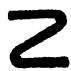
\includegraphics[keepaspectratio]{images/part001_f875b0ae.jpg}}

Remark. In a non-Hausdorff space, a compact set need not be closed, and its closure need not be quasi-compact (Exercise 5); the intersection of two compact sets need not be quasi-compact (Exercise 5); the union of two compact sets need not be compact (Exercise 5).

